\documentclass[11pt]{article}
\usepackage[french]{babel}
\usepackage[T1]{fontenc}
\usepackage{fontspec}
\usepackage[utf8]{inputenc}
\usepackage{url}
\usepackage{eurosym}
\usepackage{pdfpages}
\usepackage{ulem} % to use a strikeout/strikethrough font
\usepackage{color}
\newcommand{\fs}[1]{\textcolor{red}{\sout{#1}}}
\newcommand{\f}[1]{\textcolor{blue}{#1}}
\usepackage{graphicx} % Inclure des images
\usepackage{multicol} % Multi-colonnes


\usepackage[autolanguage, np]{numprint} % écriture des virgules
\usepackage[top=3cm,right=2cm,bottom=2cm,left=2cm]{geometry}

\title{HAUM}
\author{Assemblées Générales Ordinaire \& Extraordinaire}
\date{A définir 2022}

\begin{document}
\maketitle

\section*{Convocation}

Madame, Monsieur,

L'association HAUM vous convoque à ses Assemblées Générales Ordinaire \& Extraordinaire qui se tiendront le :

\begin{center}
{\Large A définir 2022 à 19h00}\\
à Le Mans Innovation, \\57 Bd Demorieux au 2\textsuperscript{ème} étage, \\72 100 Le Mans
\end{center}

En cas d'impossibilité, veuillez vous faire excuser et vous faire représenter si vous le souhaitez (2 procurations maximum par personne présente, Statuts, art. 6).

\newpage

\hrule
\vspace{.6cm}
\begin{center}
\Large\bfseries Assemblée Générale Ordinaire
\end{center}
\vspace{.3cm}
\hrule

\vspace{1.5cm}

\section*{Déroulement}

\begin{enumerate}
    \item Présentation de l'association
    \item Rapport moral
        \begin{enumerate}
            \item Bilan
            \item Objectifs
            \item Questions
        \end{enumerate}
    \item Rapport financier
        \begin{enumerate}
	    \item En images
            \item Bilan \& Objectifs
            \item Questions
        \end{enumerate}
    \item Motions et vote
    \item Élection du nouveau bureau
    \item Questions diverses
\end{enumerate}

Vous trouverez en annexe au présent document le budget prévisionnel 2022.

\section{Présentation de l'association}

\section{Rapport Moral}

\subsection{Bilan}

\subsubsection{Le Mans Innovation \& déménagement}

\subsubsection{Evènements}

\paragraph{NomDeL'évènement} Sur une invitation de l'Électrolab (Nanterre), le HAUM a participé à
HAMExpo, salon de radioamateurs organisé au Mans en 2018. Les membres présents ont pu
échanger avec la communauté des RA et avec quelques membres de l'Électrolab.

\subsubsection{Projets et axes}

Il y a plusieurs projets en cours. Au niveau collectif (pour des projets qui occupent
quelques personnes) on a aujourd'hui:

\begin{description}
	\item[Photographie] Sténopé, stéréo-photographie, etc\ldots
	\item[Lumière] Plusieurs projets également : scratch holograms, light painting,  moirés, Tål
	\item[IdiHAUM\footnotemark]\footnotetext{Nom non définitif} Solution de contrôle d'accès
\end{description}

Les réunions "projets" qui avaient été proposées et instaurées lors de la dernière années
ont été plutôt bien suivies et utiles au début de l'exercice et ont complètement disparu
pendant l'été. Elle permettaient à tous de s'informer des projets en cours régulièrement
et une solution de remplacement est peut être à chercher.

\subsection{Objectifs}

\section{Rapport financier}

\subsection{En images}
Nous présentons ici le bilan financier de l'année 2017.
\begin{center}
%\begin{multicols}{2}
%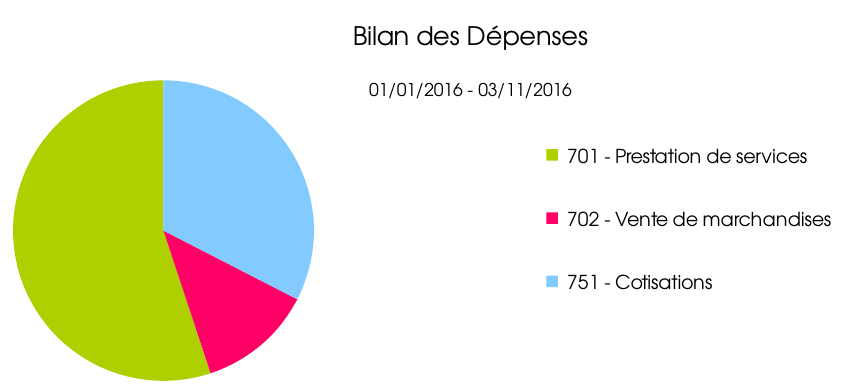
\includegraphics[width=8cm]{1DossierAGRecettes.png}

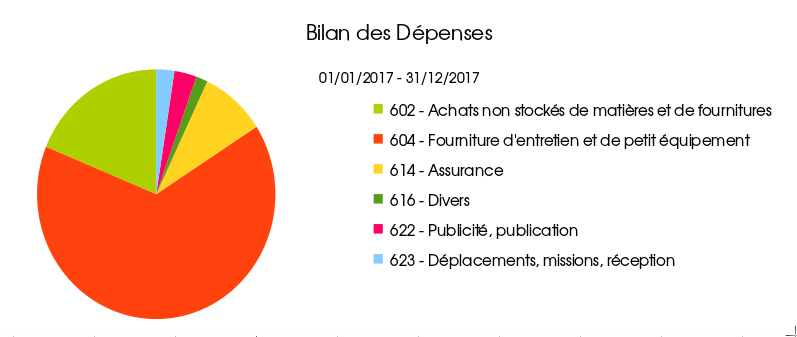
\includegraphics[width=8cm]{2DossierAGDepenses2017.png}
%\end{multicols}

\begin{multicols}{2}
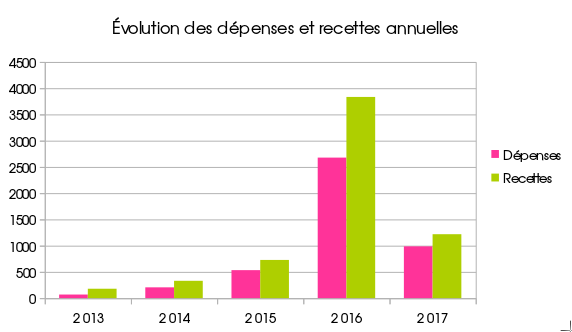
\includegraphics[width=8cm]{3DossierAGGeneral2017.png}

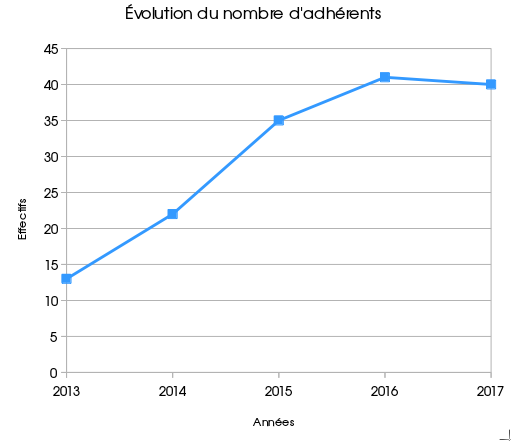
\includegraphics[width=8cm]{4DossierAGAdherents2017.png}
\end{multicols}
\end{center}
\subsection{Bilan et objectifs}
Après une année 2016 en forte croissance, il y a eu une stabilisation des volumes
financiers en 2017.

Dans la continuité de l'an passé, nous avons poursuivi l'objectif de mutualisation
des moyens matériel. Le Mans Innovation nous a mis à disposition une découpeuse laser
dans notre local et nous avons investi dans une machine à tricoter, un routeur
et une Kress.

Si on souhaite être en capacité de financer des machines ou de l'outillage plus onéreux
ou en plus grand nombre, l'augmentation des cotisations, des mécénats et/ou des
actions qui seraient capables de nous rapportés de l'argent seraient les bienvenus.

Cette année, les dépenses ont été effectuées en suivant rigoureusement les règles
instaurées depuis 2 ans maintenant. La gestion de trésorerie fut donc plus aisée.

Pour continuer dans cette dynamique, nous rappelons ici les règles de fonctionnement :
\begin{itemize}
 \item toutes les factures doivent être établies \textbf{au nom du HAUM} et ne
 contenir que des éléments \textbf{achetés pour le HAUM} ;
 \item les dépenses de l'argent du hackerspace ne doivent être faites qu'après
 \textbf{consultation des autres membres} et, surtout, \textbf{vérification de la
 trésorerie} ;
 \item une demande de validation \textbf{par mail} doit être effectuée.
\end{itemize}

Le bilan financier contient, à ce jour, deux impayés : un premier de 250\euro{}
(concernant un chèque refusé à trois reprises) et un second de 300\euro{} (Prestation
Teriaki).

\paragraph{Prévisions 2018}
Pour l'année à venir, le budget prévisionnel a été construit sur la base des charges
et des recettes de l'année 2017.

\subparagraph{Recettes}
Il est estimé pour les recettes :
\begin{itemize}
 \item 300\officialeuro~ de prestations ;
 \item 1200\officialeuro~ de cotisations.
\end{itemize}

\subparagraph{Charges}
Pour les charges, il est prévu :
\begin{itemize}
 \item 265\officialeuro~ pour l'achat de fournitures ;
 \item 700\officialeuro~ pour les petits équipements ;
 \item 246\officialeuro~ pour les autres fournitures (par exemple, en 2016, les tee-shirts) ;
 \item 50\officialeuro~ pour la communication (cartes de visites, ...) ;
 \item 150\officialeuro~ pour les frais de déplacement, de réception, ...
\end{itemize}

\subparagraph{Bénévolat}La valorisation du bénévolat sera établie régulièrement lors des réunions mensuelles.
Elle a été estimée à \np{8142}\officialeuro~ pour l'année prochaine.

\subparagraph{}Le budget prévisionnel est alors de \np{18942}\officialeuro.

\section{Motions}
Aucun amendement au Règlement Intérieur n'a été proposé.

\section{Questions Diverses}

\newpage

\hrule
\vspace{.3cm}
\begin{center}
\Large\bfseries Assemblée Générale Extraordinaire
\end{center}
\vspace{.3cm}
\hrule

\vspace{1.5cm}

\section*{Déroulement}

\begin{enumerate}
    \item Appel et annonce des procurations
		\item Questions diverses
\end{enumerate}

\section*{Clotûre}

\newpage

\clearpage
\thispagestyle{empty}
\topskip0pt
\vspace*{\fill}
\begin{center}
\hrule
\vspace{.3cm}
\Huge\bfseries Annexes
\vspace{.3cm}
\hrule
\vspace{2cm}
\Large
\noindent Budget Prévisionnel 2018
\end{center}
\vspace*{\fill}

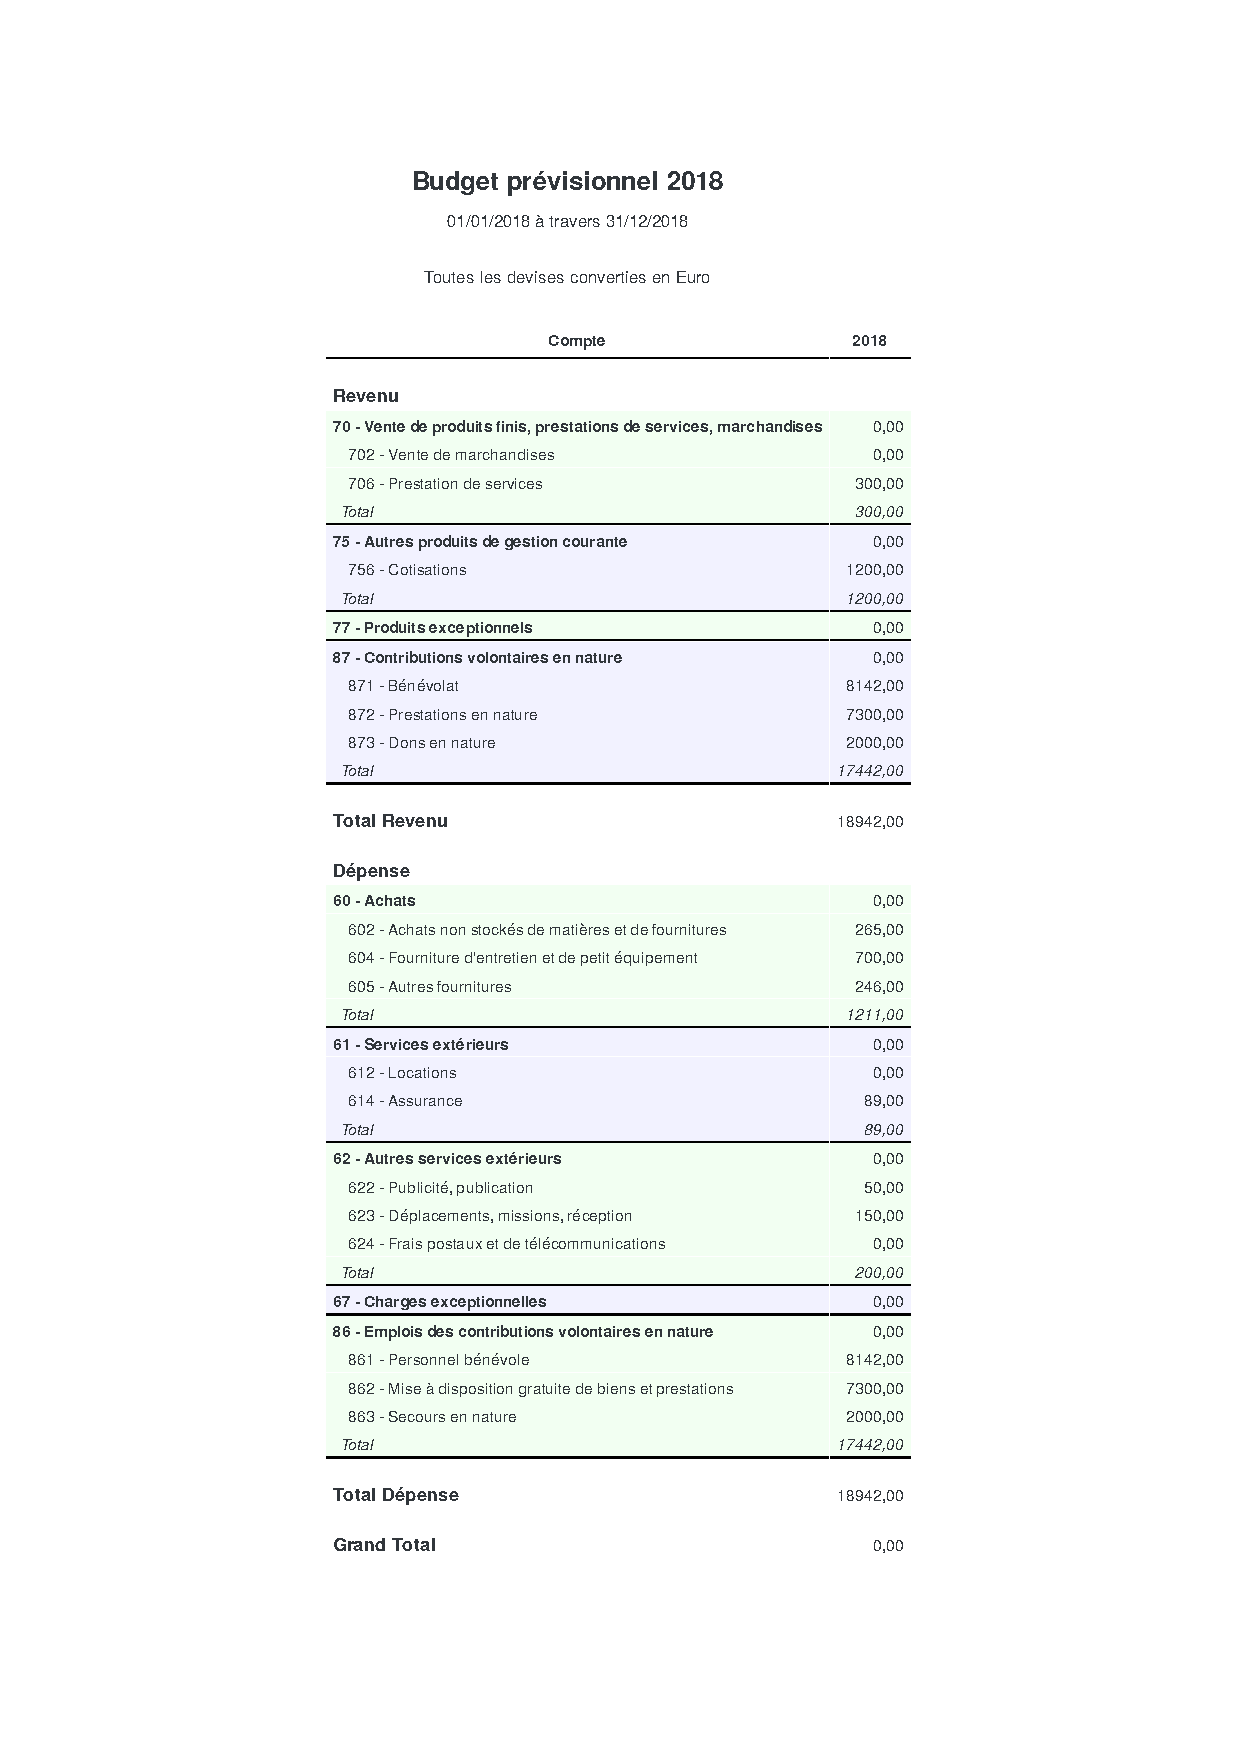
\includepdf[pages=-]{BudgetPrevisionnel2018.pdf}

\end{document}

% vim: set spelllang=fr:
